\chapter{Physics Objects}


\section{Particle Flow (PF) }

The global event reconstruction (also called particle-flow event reconstruction \cite{PF1, PF2, PF3}) consists in reconstructing and identifying each single particle with an optimized combination of all subdetector information.

In this process, the identification of the particle type (photon, electron, muon, charged hadron, neutral hadron) plays an important role in the determination of the particle direction and energy.
 
\begin{itemize}
 \item \textbf{Photons}
(\eg coming from \Pgpz  decays or from electron bremsstrahlung) are identified as ECAL energy clusters not linked to the extrapolation of any charged particle trajectory to the ECAL. The energy of photons is directly obtained from the ECAL measurement, corrected for zero-suppression effects.

\item \textbf{Electrons} 
(\eg coming from photon conversions in the tracker material or from \cPqb-hadron semileptonic decays) are identified as a primary charged particle track and potentially many ECAL energy clusters corresponding to this track extrapolation to the ECAL and to possible bremsstrahlung photons emitted along the way through the tracker material. The energy of electrons is determined from a combination of the track momentum at the main interaction vertex, the corresponding ECAL cluster energy, and the energy sum of all bremsstrahlung photons attached to the track.

\item \textbf{Muons}
 (\eg from \cPqb-hadron semileptonic decays) are identified as a track in the central tracker consistent with either a track or several hits in the muon system, associated with an energy deficit in the calorimeters. The energy of muons is obtained from the corresponding track momentum.
 
\item \textbf{Charged hadrons} 
are identified as charged particle tracks neither identified as electrons, nor as muons. The energy of charged hadrons is determined from a combination of the track momentum and the corresponding ECAL and HCAL energy, corrected for zero-suppression effects and for the response function of the calorimeters to hadronic showers.

\item \textbf{Neutral hadrons}
are identified as HCAL energy clusters not linked to any charged hadron trajectory, or as ECAL and HCAL energy excesses with respect to the expected charged hadron energy deposit. The energy of neutral hadrons is obtained from the corresponding corrected ECAL and HCAL energy.
\end{itemize}

\begin{figure}[htp]
  \centering
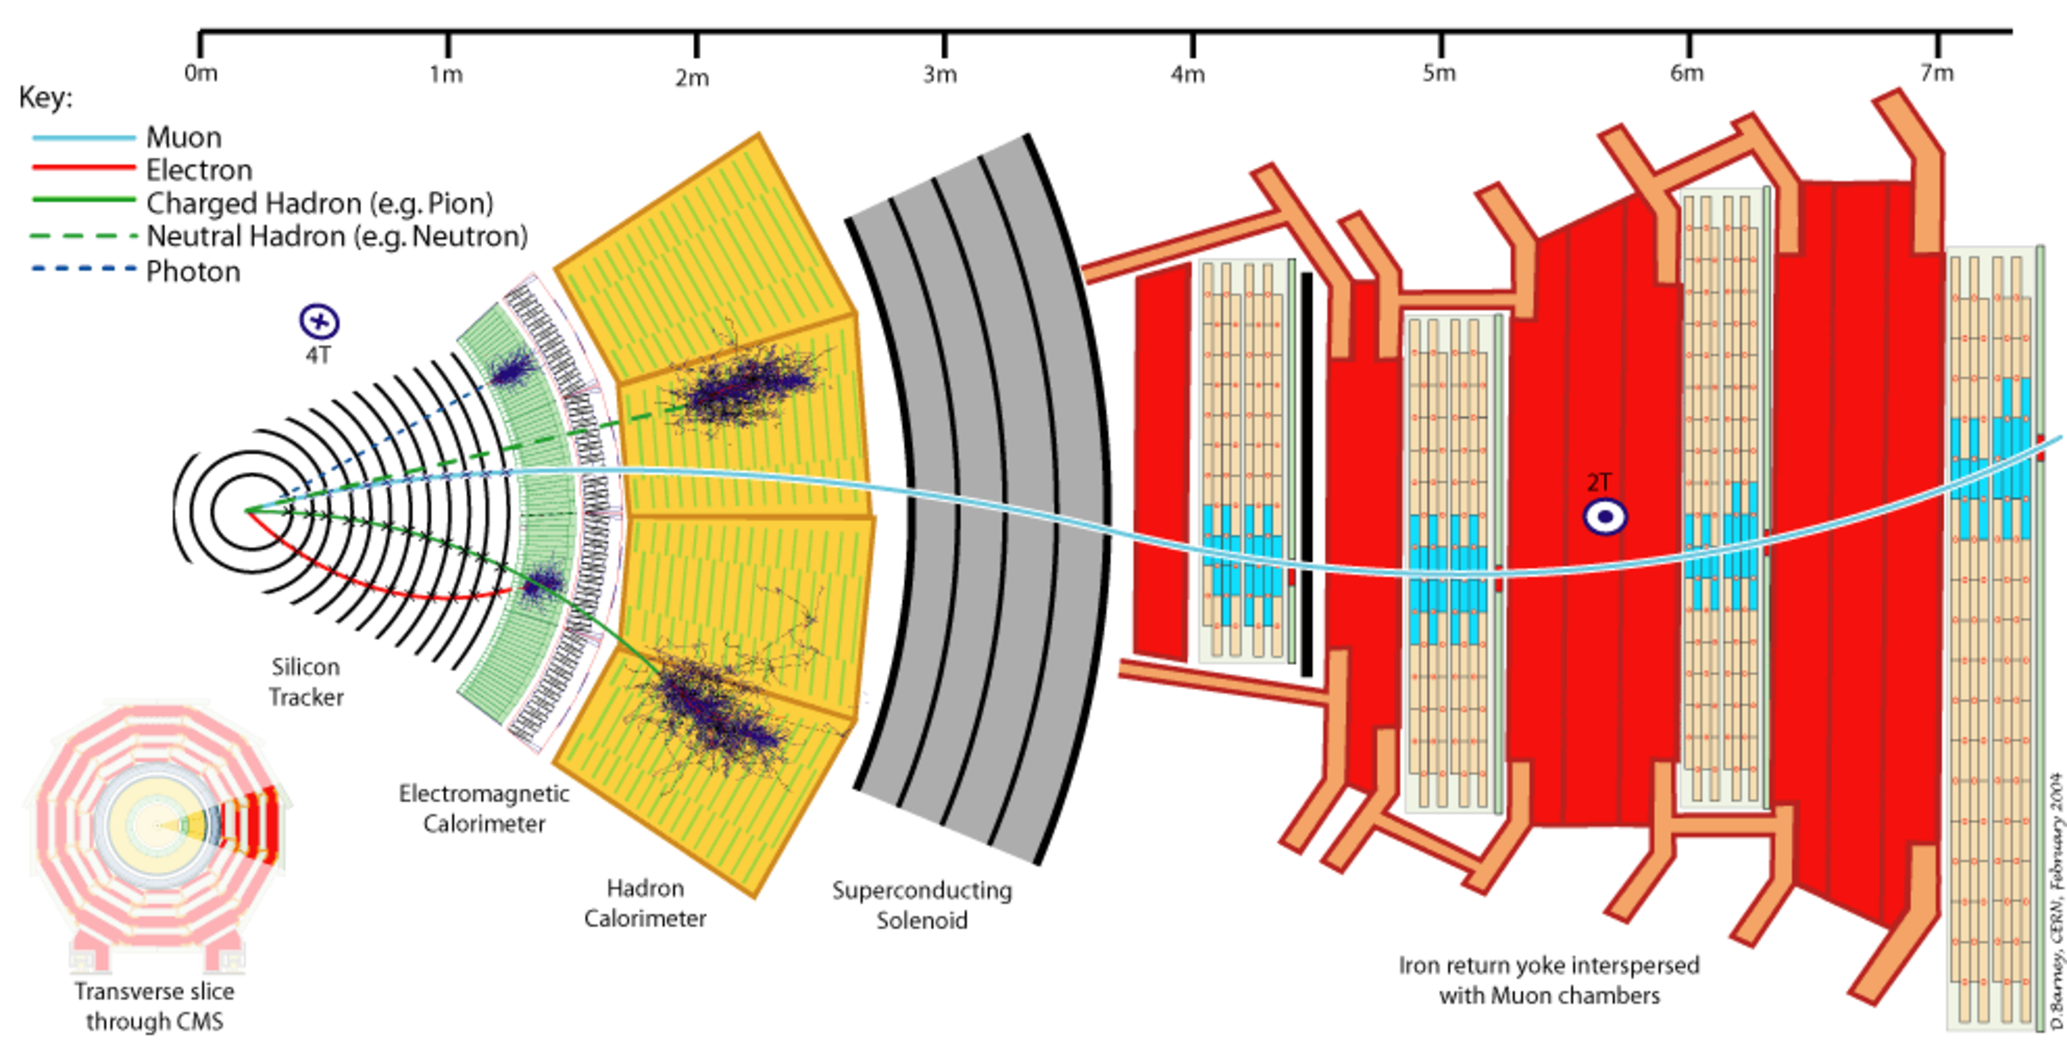
\includegraphics[width=16cm]{CMS_chapter_plots/CMS_Slice}
\label{figure}\caption{CMS Detector transverse slice}
\end{figure}

\section{Jets }\label{aniktlab}

Jets are the experimental signatures of quarks and gluons produced in high-energy processes such as hard scattering of partons in proton-proton collisions.

The LHC collides protons containing colored partons: quarks, antiquarks and gluons. Almost immediately after being produced, a quark or gluon fragments and hadronises, leading to a collimated spray of energetic hadrons: a jet (Fig. \ref{jet1figure} ).
\begin{figure}[H]
  \centering
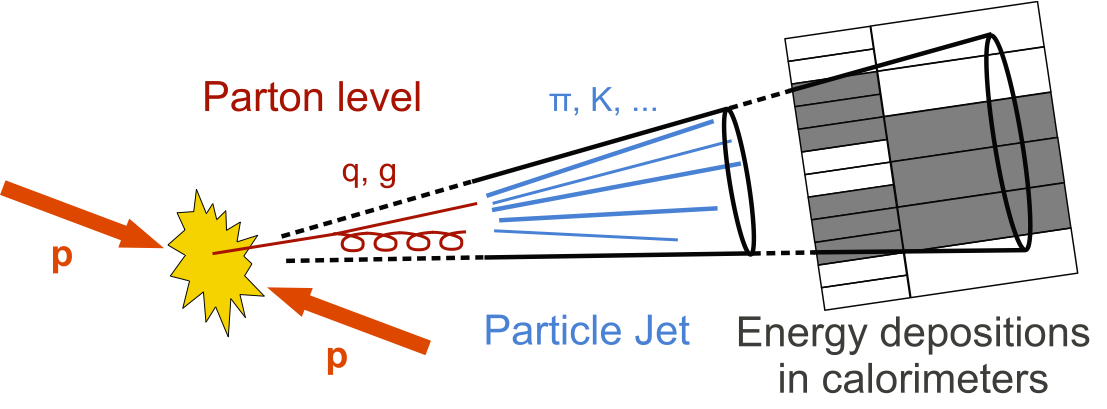
\includegraphics[width=12cm]{physics_objects_plots/Jet1}
\caption{pp-collision resulting in a collimated spray of particles, a jet. \label{jet1figure}}
\end{figure}

Jets are obvious structures when one looks at an event display,
and by measuring their energy and direction one can get close to
the idea of the original parton (Fig. \ref{jet2figure}).
\begin{figure}[H]
  \centering
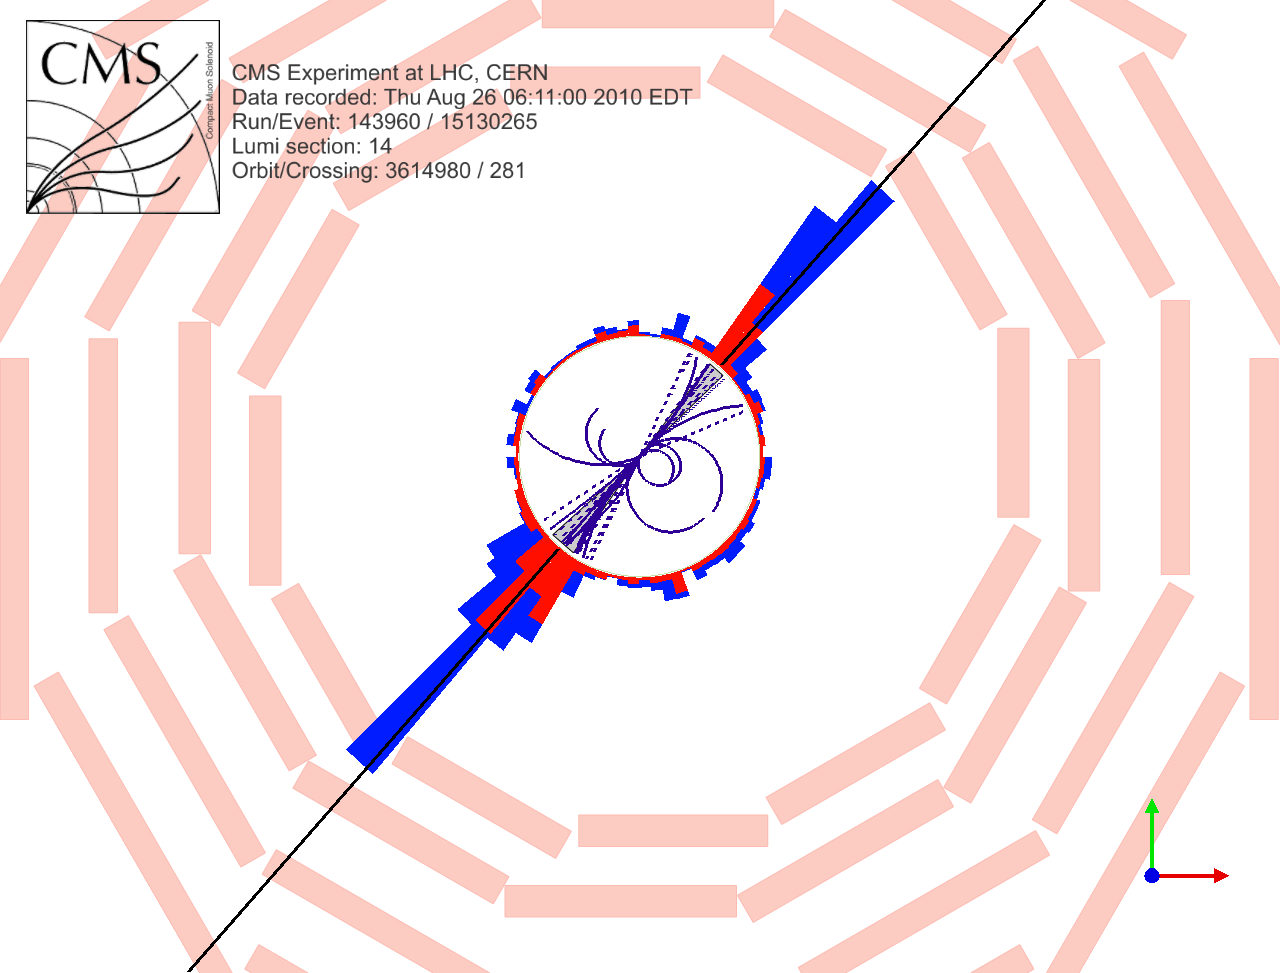
\includegraphics[width=8cm]{physics_objects_plots/Jet2}
\caption{CMS event display for a dijet reaction \label{jet2figure}}
\end{figure}

Jet clustering algorithms provide a set of rules for grouping particles into jets. They usually involve one or more parameters that indicate how close two particles must be for them to belong to the same jet.

Additionally they are always associated with a recombination scheme, which indicates what momentum to assign to the combination of two particles.

Taken together, a jet algorithm with its parameters and a recombination scheme form a jet definition.
There are many types of jet algorithms in the market, but in run-2 CMS will mainly use the anti-kt algorithm \cite{antikt}.
First we introduces the distances $d_{ij}$ between entities (particles, pseudojets) $i$ and $j$ and $d_{iB}$ between entity
$i$ and the beam (B). The (inclusive) clustering proceeds by identifying the smallest of the distances and if it is a $d_{ij}$ recombining entities $i$ and $j$, while if it is $d_{iB}$ calling
$i$ a jet and removing it from the list of entities. The distances are recalculated and the procedure repeated until no entities are left. The definitions:
\begin{eqnarray}
d_{ij} &=& \text{min}\left(k^{2p}_{ti},k^{2p}_{tj} \right) \dfrac{\Delta^{2}_{ij}}{\Delta R^{2}}\\
d_{iB} &=& k^{2p}_{ti}
\end{eqnarray}

where $\Delta^{2}_{ij}= (y_{i}-y_{j})^{2}+(\phi_{i}-\phi_{j})^{2}$ and $k_{ti}$, $y_{i}$, $\phi_{i}$ are respectively the transverse momentum, the rapidity and the azimuth of particle $i$. $\Delta R$ is the geometrical distance $\Delta R=\sqrt{\Delta\eta^{2} + \Delta\phi^{2}}$. Note that when $p=-1$ we are on the case of  the anti-kt algorithm, which is implemented in the FastJet package \cite{fastjet}.

\subsection{Jet Energy Correction ( JEC)}\label{jec}

Jet energy corrections need to be applied to account for the non-linear and non-uniform response of the CMS calorimeters \cite{jetcorrec}. They associate, on average, the $\ptrans$ of a reconstructed jet to the $\ptrans$ of the corresponding particle jet.

Jet energy measured in the detector is typically different from the corresponding particle jet energy. The latter is obtained in the simulation by clustering, with the same jet algorithm, the
stable particles produced during the hadronization process that follows the hard interaction.

The main cause for this energy mismatch is the non-uniform and non-linear response of the CMS calorimeters. Furthermore, electronics noise and additional pp interactions in the same
bunch crossing (event pile-up) can lead to extra unwanted energy. The purpose of the jet energy correction is to relate, on average, the energy measured in the detector to the energy of the corresponding particle jet.

CMS uses a factorized multi-level jet correction, shown schematically in Fig. \ref{jet3figure}, in
which the correction must be applied in the following fixed sequence:
\begin{enumerate}
\item 
\textbf{L1:Offset}: Required correction for pile-up and electronic noise.
\item
\textbf{L2:Relative} ($\eta$): Required correction for variations in jet response with pseudorapidity relative to a control region.
\item
\textbf{L3:Absolute} ($p_{T}$): Required correction to particle level versus jet pT in the control region.
\item
\textbf{EMF}: Optional correction for variations in jet response with electromagnetic energy fraction.
\item
\textbf{Flavor}: Optional correction to particle level for different types of jets (light quark, c, b, gluon).
\item
\textbf{Underlying Event}: Optional correction for underlying event energy due to soft interactions involving spectator partons.
\item
\textbf{Parton}: Optional correction to parton level.
\end{enumerate}
\begin{figure}[H]
  \centering
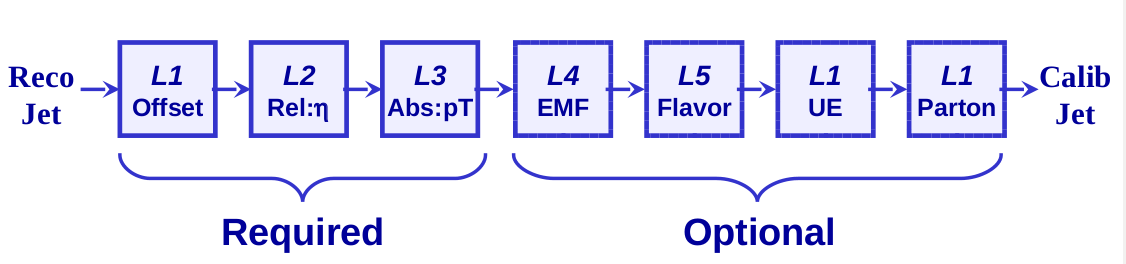
\includegraphics[width=13cm]{physics_objects_plots/jetcorr2}
\caption{Schematic picture of the factorized multi-level jet correction. \label{jet3figure}}
\end{figure}
Factorization facilitates the use of data-driven corrections, breaking the correction into pieces that are naturally measured in collider data. Combined correction brings back the jet to the particle level.

\subsection{Particle Flow Jet (PFJet)}

The Particle-Flow (PF) jets \cite{pfjet} are reconstructed by clustering the four-momentum vectors of particle-flow candidates. 

The particle-flow algorithm combines the information from all
relevant CMS sub-detectors to identify and reconstruct all visible particles in the event, namely muons, electrons, photons, charged hadrons, and neutral hadrons.

The energy of charged hadrons is determined from a combination of the track momentum and the corresponding ECAL and HCAL energy, corrected for zero-suppression effects, and calibrated for the non-linear response of the calorimeters.

The energy of neutral hadrons is obtained from the corresponding calibrated ECAL and HCAL energy. The PF jet momentum and spatial resolutions are greatly improved with respect to calorimeter jets, as the use of the tracking detectors and of the high granularity of ECAL allows resolution and measurement of charged hadrons and photons inside a jet, which together constitute $\sim$ 85$\%$ of the jet energy.

\subsubsection{Charged hadron subtraction (CHS)}

Contamination to the jet from pileup degrades the ability to reconstruct the jet observables. Previous pile up corections applied in Run I help to correct the four-vector of the jet but not
the jet structure observables.

One new approach is use tracking information which takes advantage of the fact that a large fraction of the pileup vertices are separated in space from the vertex of interest. Therefore, charged particles from pileup vertices can be removed from the jets, in a process called "charged hadron subtraction" (CHS) (Fig. \ref{jetchsfigure}).

Charged Hadron Subtraction (CHS) is a technique used to reduce the effect of "in-time pileup" on reconstructed physics objects. In this approach, charged hadrons unambiguously associated
to pileup vertices are removed from the event and the remaining PF candidates are allowed to cluster to form jets \cite{pileupchs}.
\begin{figure}[H]
  \centering
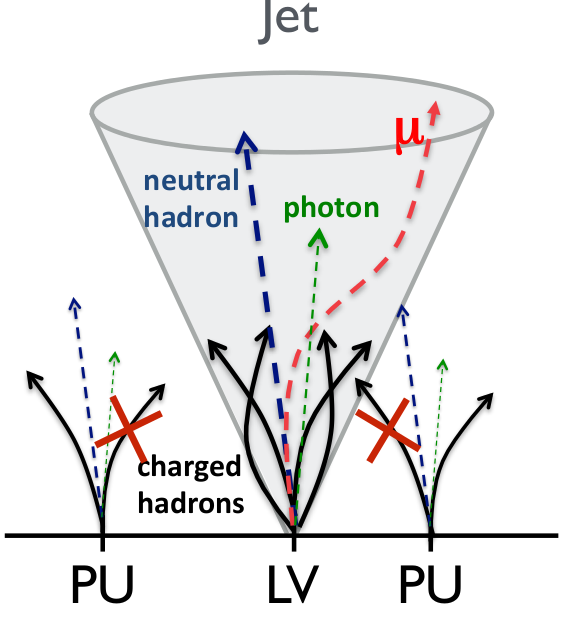
\includegraphics[width=6cm]{physics_objects_plots/chs}
\caption{Charged hadron subtraction. \label{jetchsfigure}}
\end{figure}

\subsection{V-tagging}

Generally, V tagging methods (V=Z,W weak vector boson) have depended largely on leptonic decay channels. Hadronic signatures
deal with the relatively poorer reconstruction of jets and large multijet backgrounds from QCD processes at hadron colliders.

Several recent developments have improved the tagging of hadronically decaying weak vector bosons. Many of these advances have resulted from the analysis of the internal components
of a jet, i.e. its substructure.

A more effective identification of hadronic V decays allows many analyses to profit from the substantially larger branching fraction of hadronic channels. This,
in turn, may provide significant gains in searches for new physics \cite{vtagging}.

\subsubsection{Unresolved jets}

For highly boosted weak vector bosons, the hadronic decay products can be merged into a single jet. For distance parameter R = 0.8, this occurs for boson pT above 200 GeV. The radiation profile of the individual, hard partons within a merged jet must be explicitly resolved for an accurate calculation of the boson mass. 

This contrasts with the resolved scenario, for which the boson mass can be determined simply from the properties of the individually reconstructed jets.

A new class of observables has been developed for disentangling the radiation profiles of proximate partons. We explore these observables in this section.

Jet mass is the most natural discriminator between jets originating from V decays and those originating from single partons. Jet grooming techniques improve mass resolution by reducing the effects from pileup and underlying event. The following grooming algorithms are studied:

\paragraph{N-subjetiness}\label{tau21sec}
This method uses the distribution of jet constituents relative to the jet axis in order to quantify how well the jet can be divided into N subjets.

The computation is done by reclustering the jet using the kT-algorithm until N protojets are left. The direction of the remaining jets are then used to compute the "N-subjetiness" as
\begin{eqnarray}
\tau_{N}=\dfrac{1}{d_{0}} \sum_{k}\: p_{T,k}\times \text{min}\left( \Delta R_{1,k}, \Delta R_{2,k},\dots,\Delta R_{N,k}\right) 
\end{eqnarray}
with the normalization factor $d_{0}$ :
\begin{eqnarray}
d_{0} = \sum_{k} p_{T,k}\times R_{0}
\end{eqnarray}
and $R_{0}$ is the clustering parameter of the original jet, $p_{ T,k}$ is the pT of the k-th jet constituent and $\Delta R_{n,k}$ is its distance to the n-th subjet. In particular, the ratio of the "2-subjettiness" to the "1-subjettiness" $(\tau_{2} / \tau_{1} = \tau_{21} )$ has excellent capability at separating jets originating from boosted vector bosons from jets originating from quarks and gluons \cite{subjetiness}.
\begin{figure}[H]
  \centering
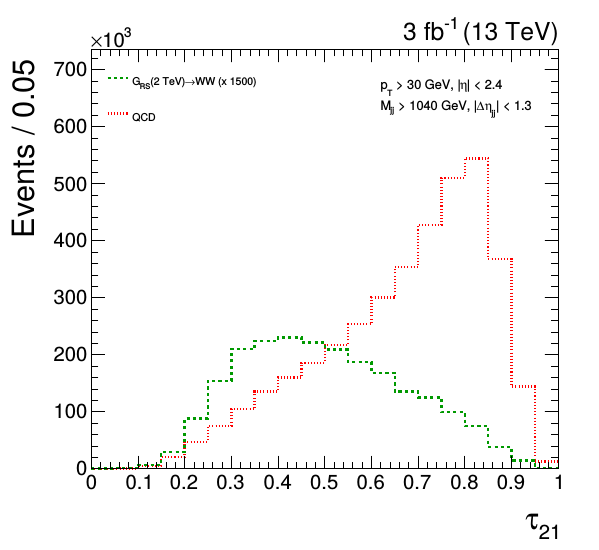
\includegraphics[width=8cm]{physics_objects_plots/tau21}
\caption{$\tau_{21}$ distribution for signal and background \label{jettau21figure}}
\end{figure}

\paragraph{Pruning}\label{prun}
This method \cite{pruning} attempts to isolate subjet showers by removing soft, large angle particles from each subjet. Pruning will remove the uncorrelated contributions from underlaying events and pile up that make significant contributions to the jet mass.

The mass of the resulting pruned jet is small if we start with a QCD jet, and near the particle mass if we start with a jet containing the decay products of a heavy particle. 
%Procedure: Define parameters $z_{\text{cut}}$=0.1 and $r_{\text{cut}}=0.5$. Reclustering with sequential recombination algorithm (CA), veto soft and large-angle recombination between pseudojets $i$ and $j$:
\begin{eqnarray}
\Delta R_{ij}> r_{\text{cut}}\times\dfrac{2m}{p_{T}},\ \ \  \ \  z=\text{min}\left( \dfrac{p_{Ti}, p_{T_{j}}}{p_{T_{i+j}}} \right) < z_{\text{cut}}  
\end{eqnarray}

\begin{figure}[H]
  \centering
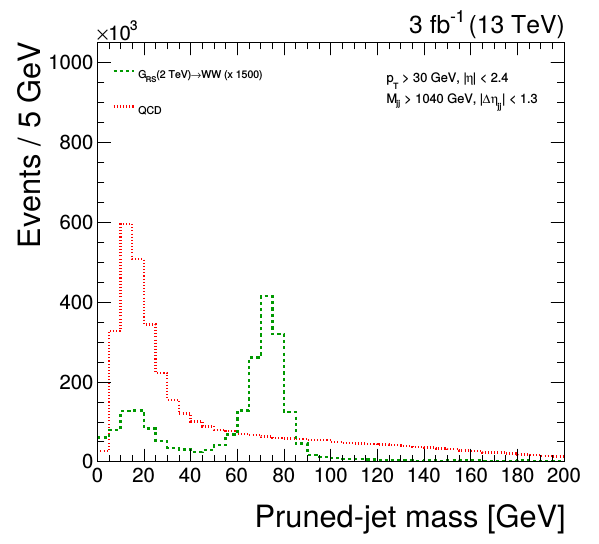
\includegraphics[width=8cm]{physics_objects_plots/prun}
\caption{Pruned mass distribution for signal and background \label{jetprunfigure}}
\end{figure}


\section{Missing Transverse Energy ($\met$) }\label{MET1}

Missing transverse momentum plays a critical role in many physics analyses at the LHC. It is a key variable in many searches for physics beyond the standard model, such as extra dimensions and supersymmetry as well as for collider dark matter searches.

Some neutral particles which interact weakly with matter ( \ie   neutrinos ) leave the detector without producing any direct response in the detector components. The presence of such particles (also called invisible particles, Fig. \ref{figuremet1}) must be implied from the imbalance of total momentum considering that the detector is hermetic. The vector momentum imbalance in the plane perpendicular to the beam direction is particularly useful in $\cPp\cPp$ and $\ppbar$ colliders, and is known as missing transverse momentum, here denoted $\vec{\met}$ . Its magnitude is called missing transverse energy, and is denoted $\met$ (MET).


\begin{figure}[H]
  \centering
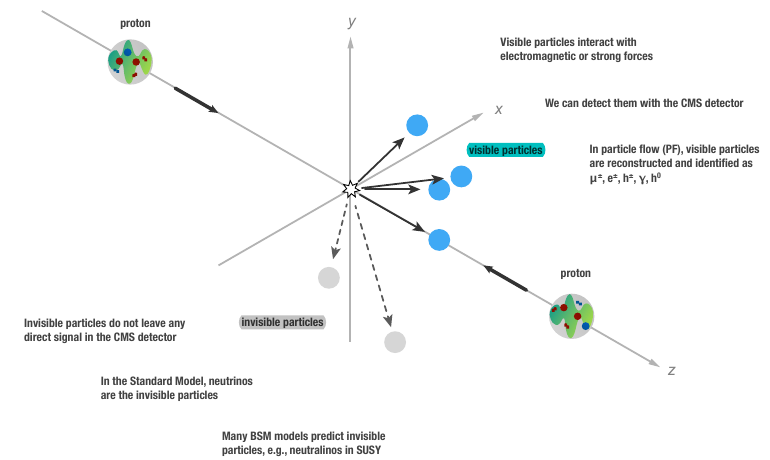
\includegraphics[width=14cm]{physics_objects_plots/met_rec}
\caption{Invisible and visible particles \label{figuremet1}}
\end{figure}

In general $\vec{\met}$ is calculated as the negative of the vector sum of the components of momentum transverse to the beam axis of all final-state particles reconstructed in the detector. 

CMS has developed three distinct algorithms to reconstruct $\vec{\met}$. (a) Calo $\met$  based on calorimeter energies and calorimeter tower geometry \cite{CaloMET}, (b) TC $\met$ calculated by replacing the calorimeter tower energies matched to charged hadrons with their corresponding charged-track momenta \cite{TrackMET}, and (c)PF $\met$ calculated using a complete particle-flow technique \cite{PF1}. In thi work we will focus on PF $\met$.

The $\met$ reconstruction is sensitive to detector malfunctions and various reconstruction effects resulting in particle momentum mismeasurements and particle misidentification. Precise calibration of all physics objects is crucial for the $\met$ reconstruction, and $\met$ is particularly sensitive to multiple proton-proton interactions in the same, earlier, and later bunch crossings (pileup interactions). Thus, it is essential to study reconstruction in detail with data.


In Run-I, identifying and removing the causes of large fake $\met$ was the major challenge in $\met$ reconstruction at CMS. By the time Run-I ended in early 2013, it was developed a matured set of $\met$ filters to reject such large fake $\met$. These filters are used in the event selections of many physics analyses. Below is a list of the main filters \cite{FiltersMET}:
\begin{itemize}
\item 
CSC tight beam halo filter
\item
HBHE noise filter with isolated noise rejection
\item
HCAL laser filter
\item
ECAL dead cell trigger primitive (TP) filter
\item
Tracking failure filter
\item
Bad EE Supercrystal filter
\item
ECAL Laser correction filter
\item
Tracking POG filters
\end{itemize}

Some filters are used online in HLT. After the $\met$ filters are applied, the agreement of the $\met$ spectrum
with simulation, significantly improves (Fig. \ref{figuremetmiss} )
\begin{figure}[H]
  \centering
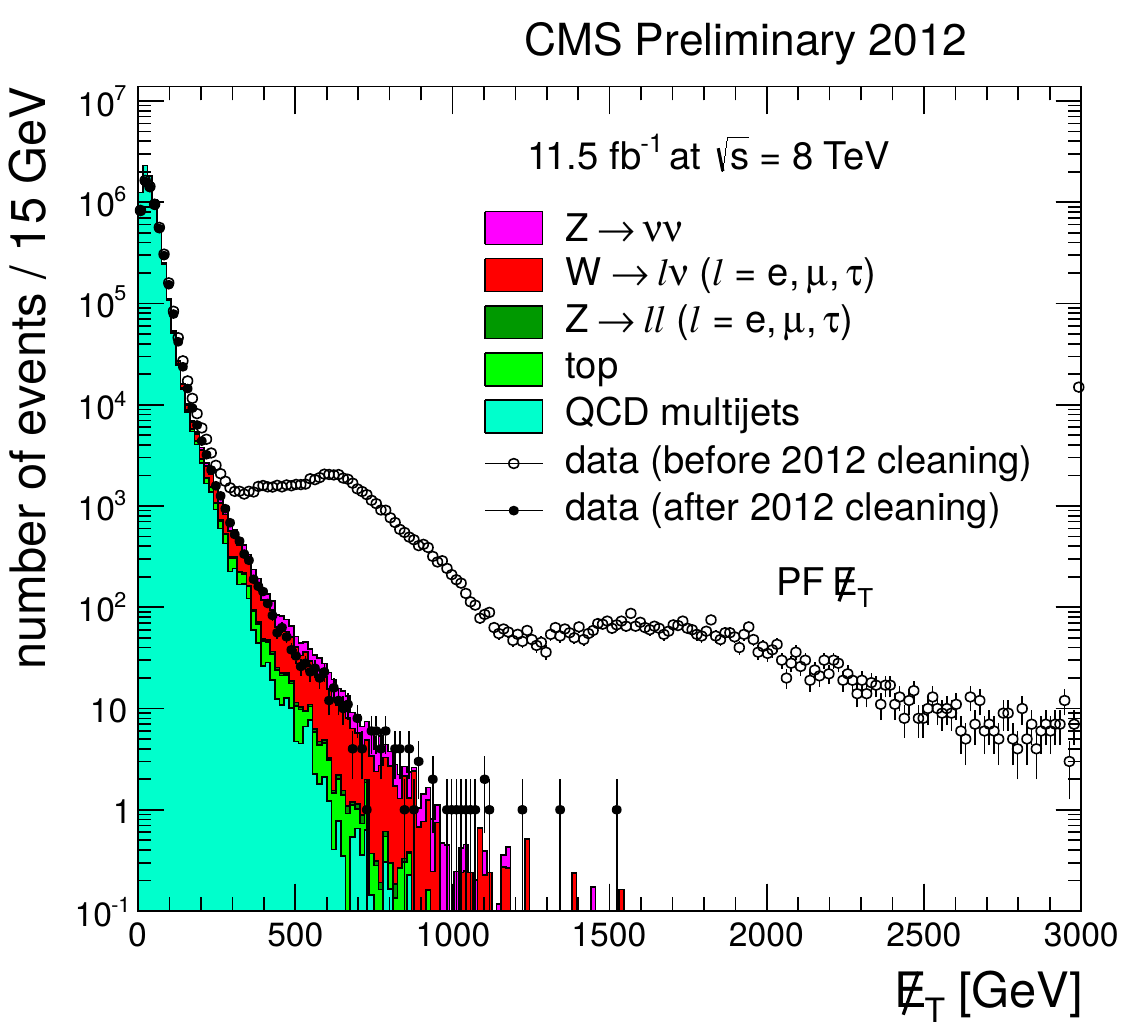
\includegraphics[width=8cm]{physics_objects_plots/met_missrec}
\caption{Comparison before and after apply the $\met$ Filters. \label{figuremetmiss}}
\end{figure}

\subsection{Particle Flow MET (PF $\met$)}

The particle flow technique aims to reconstruct a complete, unique list of particles in each event using an optimal combination of information across all CMS subdetector systems. Particles which are
reconstructed and identified include muons, electrons (with associated bremsstrahlung photons), photons (unconverted and converted), and charged and neutral hadrons.

The PF $\met$ hereafter called MET is then simply the negative vector sum of all such reconstructed particles in the event (Fig. \ref{figuremet2}).
\begin{eqnarray}
\vec{\met} = - \sum_{i \in  \text{vis.}}\:\vec{p}_{\mathrm{T}_{i}} 
\end{eqnarray}

\begin{figure}[H]
  \centering
\includegraphics[width=14cm]{physics_objects_plots/met2}
\caption{Vector sum of the reconstructed particles in the event. \label{figuremet2}}
\end{figure}

\subsection{The Type-I Correction}\label{typeI}

Raw MET is the negative of the vector sum of all reconstructed particles. The raw MET is systematically different from true MET, i.e., the transverse momentum carried by invisible particles, for many reasons including the non-compensating nature of the calorimeters and detector misalignment. To make MET a better estimate of true MET, MET corrections can be applied. 
The Type-I correction \cite{TypeIMET} is the most popular MET correction in CMS. This correction is a propagation of the jet energy corrections (JEC) to MET. The Type-I correction replaces the vector sum of transverse momenta of particles which can be clustered as jets with the vector sum of the transverse momenta of the jets to which JEC is applied. 
\begin{eqnarray}
\vec{\met}^{\text{raw}} = - \sum_{i\in \text{all}}\:\vec{p}_{\,\mathrm{T}_{i}} 
\end{eqnarray}
\noindent
The particles can be classified into two disjoint sets: either
clustered as jets or unclustered
\begin{eqnarray}
\vec{\met}^{\text{raw}} = - \sum_{i\in \text{jets}}\:\vec{p}_{\,\mathrm{T}_{i}} - \sum_{i\in \text{uncl.}}\:\vec{p}_{\,\mathrm{T}_{i}}
\end{eqnarray}

The vector sum of $\ptrans$ of all particles clustered as jets is the same as the vector sum of $\ptrans$ of all jets.
\begin{eqnarray}
\sum_{i\in\text{jets}}\:\vec{p}^{\,\text{raw}}_{\,\mathrm{T}_{\text{jet}}} = \sum_{i\in \text{jets}}\:\vec{p}_{\,\mathrm{T}_{i}} 
\end{eqnarray}
\begin{eqnarray}
\vec{\met}^{\text{raw}} = - \sum_{\text{jet}}\:\vec{p}^{\,\text{raw}}_{\,\mathrm{T}_{\text{jet}}} - \sum_{i\in \text{uncl.}}\:\vec{p}_{\,\mathrm{T}_{i}}
\end{eqnarray}

The Type-I correction replaces the raw jet pT with the corrected jet pT
\begin{eqnarray}
\vec{C}^{\text{Type-I}}_{T}= \sum_{\text{jet}}\:\vec{p}^{\,\text{raw}}_{\,\mathrm{T}_{\text{jet}}} - \sum_{\text{jet}}\:\vec{p}^{\,\text{JEC}}_{\,\mathrm{T}_{\text{jet}}}
\end{eqnarray}

The Type-I correction is a vector term that can be added to raw MET
\begin{eqnarray}
\vec{\met}^{\text{Type-I}} = \vec{\met}^{\text{raw}} + \vec{C}^{\text{Type-I}}_{T}
\end{eqnarray}
The Type-I corrected MET can be written as
\begin{eqnarray}
\vec{\met}^{\text{Type-I}} =  - \sum_{\text{jet}}\:\vec{p}^{\,\text{JEC}}_{\,\mathrm{T}_{\text{jet}}} - \sum_{i\in \text{uncl.}}\:\vec{p}_{\,\mathrm{T}_{i}
\end{eqnarray}


\subsection{Transverse Mass}\label{transvserve}

In this analysis we perform a search in the JET + MET final state as we will discuss in detail in the next chapter. The strategy is search for an excess related with the mass of the resonance. For that reason is neccesary introduce a variable associated with this magnitude.
  
Since the invisible particles are not directly detected in the experiment, it is difficult to reconstruct the mass of the resonance. Consider a single heavy particle of mass $M$ which decays in a JET (labeled particle 1) and MET (labeled particle 2). The mass of the parent particle can be constrained with the quantity $M_{T}$ defined by \cite{PDG}:
\begin{eqnarray}
M_{T}^{2} &=& (E_{T}(1)+E_{T}(2))^{2}  - (\vec{p}_{T}(1)+\vec{p}_{T}(2))^{2}\nonumber\\
&=& E_{T}(1)^{2} + E_{T}(2)^{2} +2 E_{T}(1)E_{T}(2) -\vec{p}_{T}(1)^{2} - \vec{p}_{T}(2)^{2} -2\vec{p}_{T}(1)\cdot \vec{p}_{T}(2)\nonumber\\
\end{eqnarray}
Considering that:
\begin{eqnarray}
E_{T}^{2} = m^{2}+\vec{p}_{T}^{2},\ \   \text{and}\ \  m(1),m(2) \approx 0
\end{eqnarray}
We obtain:
\begin{eqnarray}
M_{T}^{2} = 2 \left| \vec{p}_{T}(1)\right| \left| \vec{p}_{T}(2)\right| \left(1-\cos\phi \right) 
\end{eqnarray}
Remember that: $p_{T}(1)=p_{T}^{\text{jet}},\ \   \text{and}\ \  \met=p_{T}(2)$.
Finally we get:
\begin{eqnarray}
M_{T} = \sqrt{\:2\: p_{T}^{\text{jet}}\: \met\: \left[ 1-\cos\Delta\phi\left( \text{jet}, \met\right)  \right] } 
\end{eqnarray}


